\section{Programming part}
\subsection{Question 1}
There will be no problem in making a peer-to-peer connection between peer $A$
and peer $B$, IF and only if the clients takes into account that $A$ is on the
same host as the name server. (which implies that the clients send their public IP
address and not the local ip address).

If this is not taken into account, peer $B$ will will lookup $A$ and the name
server will tell $B$ that $A$ is found at ip 127.0.0.1, which obviously cause
$B$ to fail when trying to connect.

In the case the cilents send their public ip addresses, the communication will
go like this.

The above assumes that NAT translation will in some magic way, know how to
map the clients listening port the local clint ip.

\begin{lstlisting}
peer A (alice) <--> ns: HELLO alice alice_port
ns  <--> peer A (alice): 100 CONNECTED

peer A (alice) <--> ns: LOOKUP bob
ns  <--> peer A (alice): 200 INFO bob_ip bob_port

peer A (alice) <--> peer B (bob): HELLO alice
peer B (bob) <--> peer A (alice): 100 CONNECTED

peer A (alice) <--> peer B (bob): MSG Are you single
\end{lstlisting}

\subsection{Question 2}
It is not prudent to keep unused connections open, it just takes up system
resources. On the other hand connections should be kept open to connections
that are used frequently (because the whole connection and disconnection
process add a considerable overhead to short transmissions.

We suggest implementing a peer timeout, such that connections only idle for a
certain amount of time before they are automatically closed. This way only
active connections takes up resources in the long run.

\subsection{Question 3}
We suggest a design where a new protocol command {\tt GMSG}, that facilitates
multicast chat, is implemented. This command would carry the message to be sendt
to the other participants, as well as a list of participants (or an ID of the
group chat if a setup command is also introduced). To send a group chat message
a peer would simply send the {\tt GMSG} to all other participants. This way the
nameserver does not need to hold a register of private group chats.

With this model group chats would require no handshaking or initialization, and
could be quickly created and merged. To send a reply the client may be given a
dynamically generated identifier that corresponds to the group chat. If we require
lower overhead a {\tt GSETUP} command could be introduced, generating a more static
but easier to manage group chat.

\subsection{Question 4}
We can achieve $O(lg(n))$ with flooding. Figure 2, shows how $u0$ is
broadcasting to the rest of the network consisting of the peers
$u1,u2,u3,u4,u5,u6$.

$u0$ takes the broadcast-list and splits it in half, then $u0$ sends the
message and one of the new half broadcasting lists (the receiver
is subtracted) to the first member of the lists.

This implies that $u1$ will get the message and instructions to broadcast the
message to $u2, u3$.

$u4$ will also get the message, but will get the other half broadcasting list,
containing  $u5,u6$.

$u1$ again splits the remaining list in two and because each list now only
contains one peer, only the message is send to $u2$ and $u3$. The exact same
procedure is followed by $u4$. As mentioned above a graphical illustration is
shown in Figure 2.

\begin{figure}[!h]
    \centering
    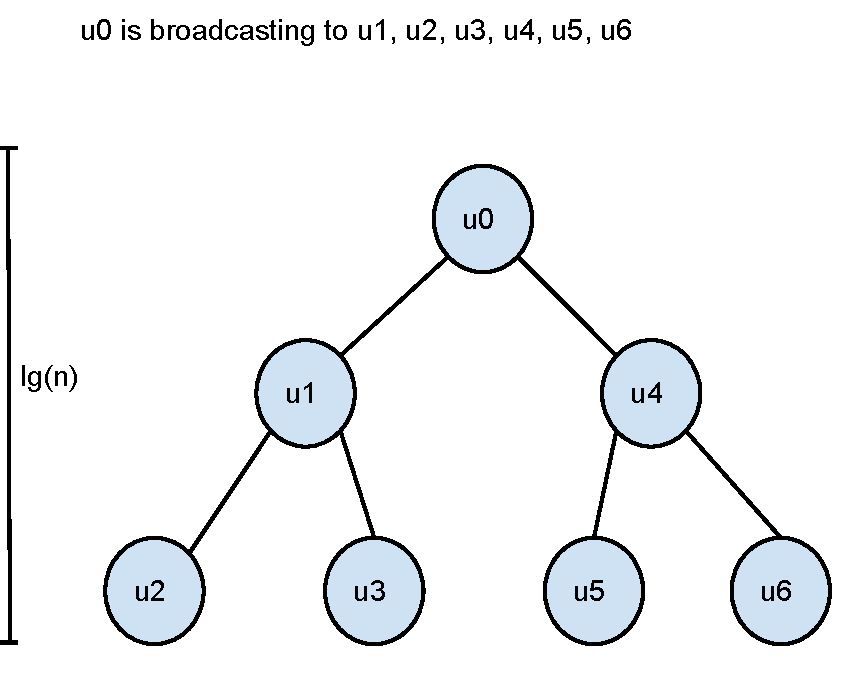
\includegraphics[width=10cm]{graphics/flooding}
    \caption{Flooding messages}
\end{figure}

\subsection{Question 5}
In regard to the name server we need the confirmation to assure that the name
server indeed removed the peer from the userlist. Even though all packages are
transmitted, the TCP protocol will not help us in case of an internal server
error etc. In that regard a missing BYE from the server tells us, that
something unexpected happened.
The same is true for the MSG ACK, this also assure us that the recipient not
only received the message, but also that it was in fact delivered to the
receivers output device.
